\section{Computer Design}

As good computer engineers, we ought to study computer
design so we can design new computers and understand
the ones that already exist.

There are two broad categories of microcontrollers,
general purpose and embedded. General purpose are
programmable and flexible. Embedded are extremely
optimized, whole-system, non-programmable application
specific devices.

The life of a silicon wafer is shown in Figure
\ref{fig:silicon}.
\begin{figure}
    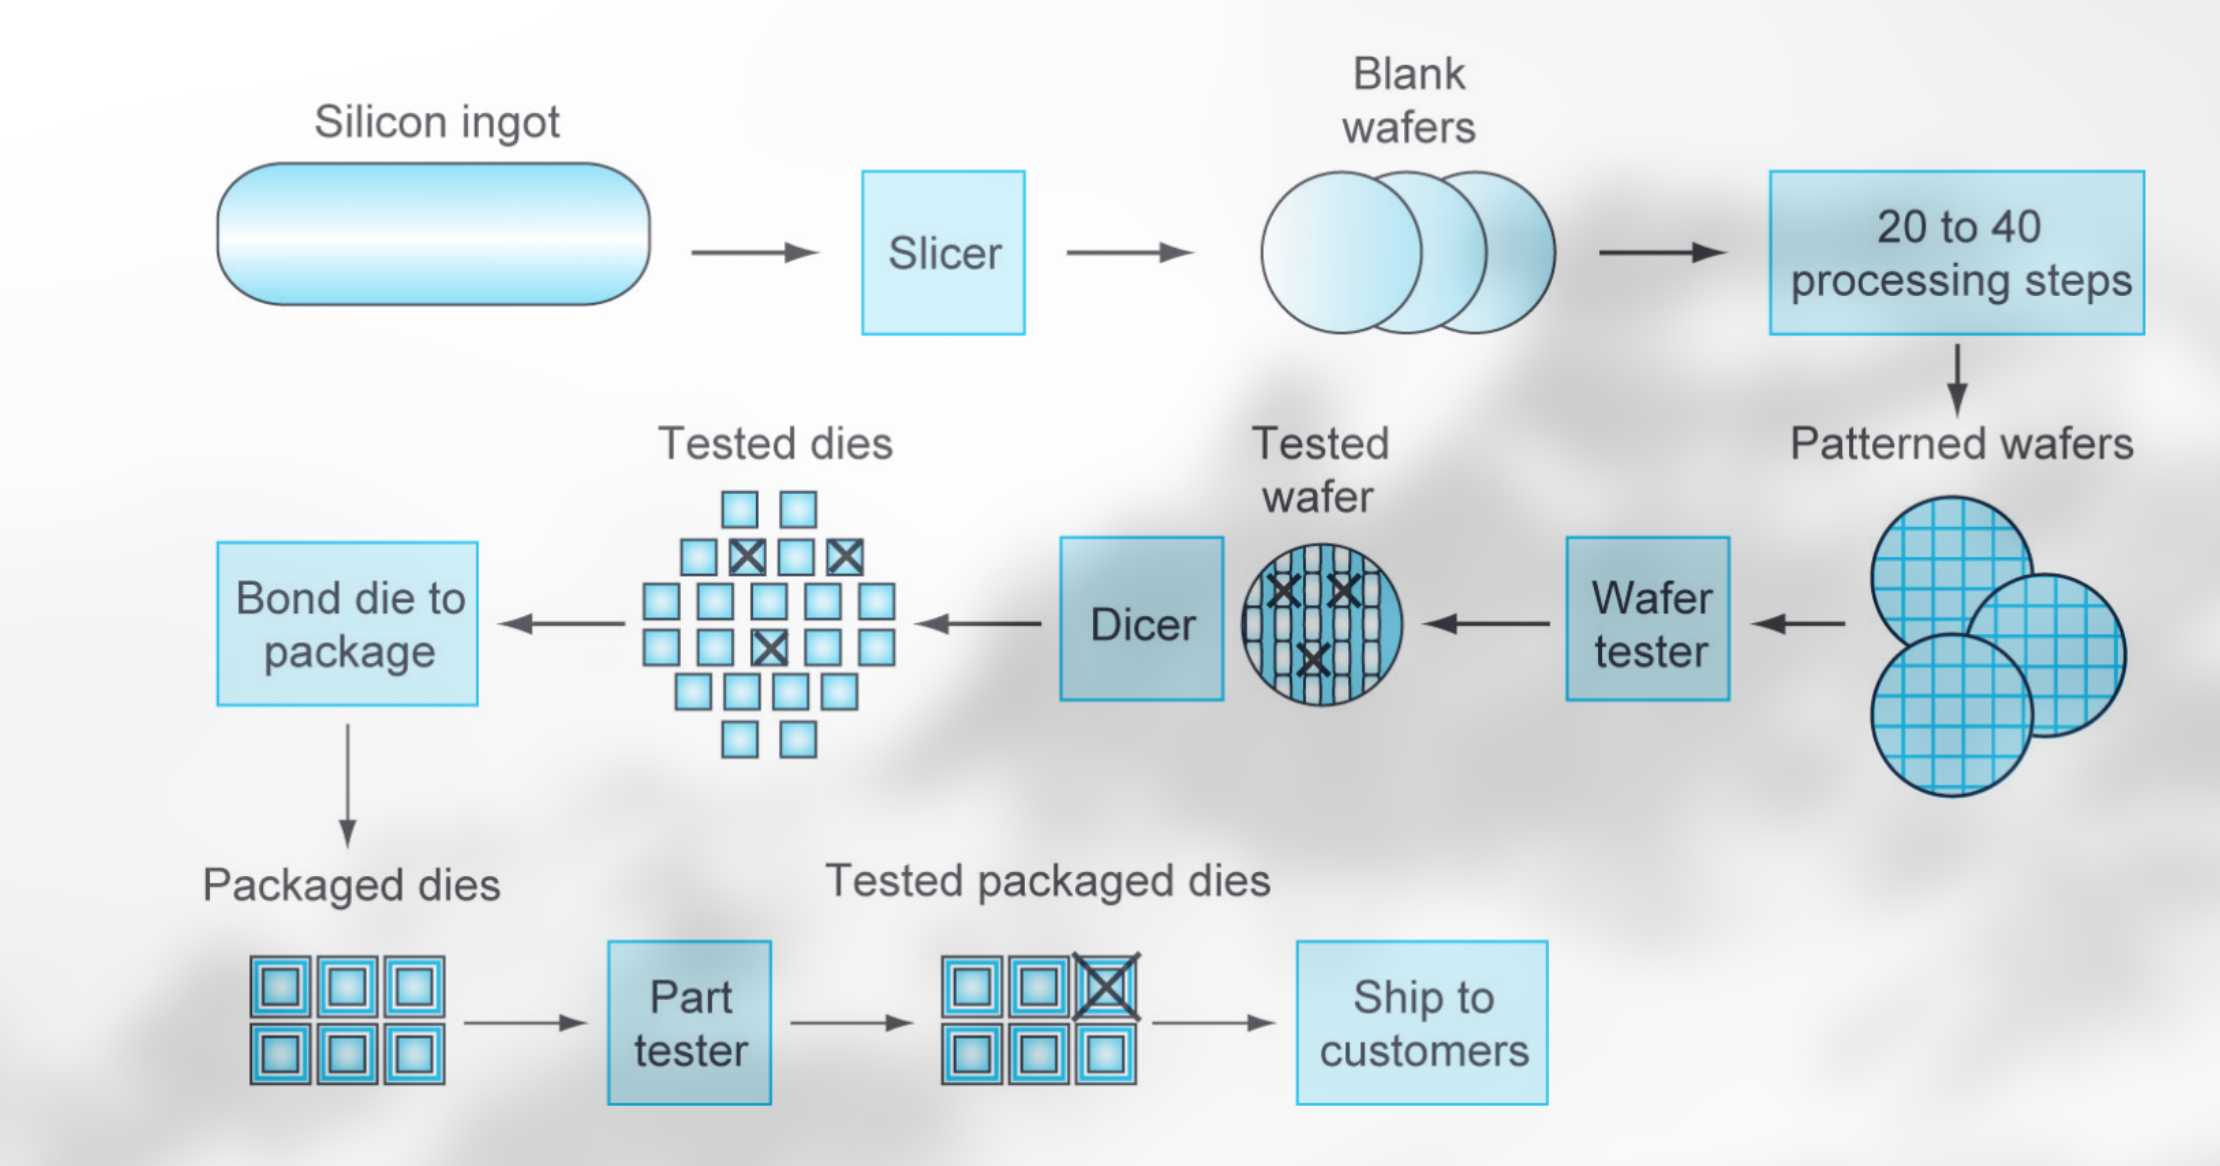
\includegraphics{images/silicon.png}
    \caption{Silicon Lifecycle}
    \label{fig:silicon}
\end{figure}
The faulty chips that fail to meet speed benchmarks
are sold as lower-grade chips in a process termed
\emph{binning}.

Even the simplest modern computers take thousands
of engineers to design. It isn't feasible to
understand everything about a computer at every
level, so we must abstract and think of the system
in terms of black boxes with inputs and outputs. This
applies to electrical engineering, computer engineering,
and programming. A high-level language like Python is
an abstraction of C, which is an abstraction of assembly
language, which is an abstraction of binary machine language.
